\documentclass[a4paper]{article}
\usepackage{amsmath, amsthm, amssymb}
\usepackage{amsfonts}
\usepackage[english]{babel}
\usepackage{fancyhdr}
\usepackage{graphicx}
\usepackage{ctable}
\usepackage{multirow}
\usepackage{url}


%For subfigures
\usepackage{caption}
\usepackage{subcaption}

%For FloatBarrier
\usepackage{placeins}


\let\oldAuthor\author


\renewcommand{\author}[1]{\newcommand{\myAuthor}{#1}\oldAuthor{#1}} 
\begin{document}
%---------------------------------------------------------
%Fill in:
%1. Title of lab. 
%2. Student names and corresponding Email addresses. If many separate 
%---------------------------------------------------------
\title{Determination of the Damping of a Pendulum with Time of Flight}
\author{Robin Lundberg (rolu0008@student.umu.se) \\ 
				Simon Ternes (sternes@students.uni-mainz.de)} 
\date{} %<-- \usepackage{amssymb, graphicx, fancyheadings} LEAVE EMPTY! 
\begin{titlepage}
\maketitle 
%---------------------------------------------------------
%Fill in:
%1. Course name
%2. Supervisor name(s), if many separate them by comma.
%-----------------------
----------------------------------
\thispagestyle{fancy}
\headheight 20pt 
\lhead{\small Department of Physics \\ Ume\aa\ University}
\rhead{\small\today}
\cfoot{Non-Invasive Measurement Techniques \\ Supervisors: Aleksandra Foltynowicz-Matyba, Bertil Sundqvist, Isak Silander, Patrick Ehlers, Amir Khodabakhsh}
\begin{abstract}
	%1. What did we do??
In this lab we measured the decay of energy in a pendulum, both from friction and air drag.
%2. experimental design
We used a laser \emph{time of flight} (ToF) method to determine the velocity--and thereby the energy---of
a pendulum; in order to examine the decay of energy against time.
%3. The results were
	%3.1 Decay
We fitted the measured decay in energy to an exponential decay model and a novel model. 
	%3.2 Air drag
The measurements with increased air drag qualitatively confirmed the theoretical expectation, however no quantitative statement could be made. 
	%3.2 Calibration
	
	%3.3 Weird damping with weight
The measured data did not fit the prediction that a heavier pendulum is damped faster, so there was an unknown factor that we could not take into account.
%4. What can we do better, conclusions.
The unknown factor of the pendulum we believe was caused by the pendulum not being completely 
constrained to move around one axis. Without this issue, the loss of energy due to friction could be better characterized.
We also didn't fit our model to a more complicated model that we derived.

\end{abstract}
\end{titlepage}
\pagestyle{fancy}
\headheight 35pt 
\rhead{\small\today}
\lhead{\myAuthor}
\cfoot{\thepage}


%\tableofcontents

\newpage
\section{Introduction}
%1. The problem in general: determine coefficient of thermal expansion of metal
%TODO

%2. Describe a bit about interferometry (Michelson interferometer) and heat expansion
%2.1 michelson interferometer
The Michelson interferometer is a common configuration for optical interferometry. A beam of light is split
into to two and made to travel different paths. The first path is used as reference and held fixed, whereas the second path is made to vary. When the beams from both these paths are joined together they will interfere with each other. The interference pattern can be measured over time and the difference in path length can be determined.
%2.2 michelson interferometer, how good is it; accuracy? 
If the path difference between the two paths changes by half the wavelength of light, we will move between two maxima in the interference pattern. So we can detect differences in path length that is less than the wavelength of light. We can also measure larger path differences by counting how many peaks you have seen.
%TODO above seems a bit not perfect

%2.2 heat expansion
%TODO

%3. How good is something today --- Dont do this

%4. Other applications --- dont do this
%TODO

%6. Our specific problem
In our lab we want to measure the coefficient of thermal expansion of unknown metal rods and from this identify what metal it is. We predict that the coefficient can be measured accurate enough to determine
what metal we are testing on. We believe that the expansion of the metal rod can be measured very exactly.
However it will not be as easy to measure the temperature of the rod since we can only measure a few points on the outside of the rod and we believe this will be the most significant source of error.


\FloatBarrier
\section{Theory}
In this lab I used five different methods to solve the one dimensional wave equation
\begin{equation}\label{eq:wave}
	\frac{\partial^2 u}{\partial t^2} = c^2 \frac{\partial^2 u}{\partial x^2}, \qquad 0\le x \le L
\end{equation}
where $c$ is the propagation speed of the wave, $u=u(x,t)$ is the displacement from equilibrium.
The initial and boundary conditions to be solved for are
\begin{equation}\label{eq:initial}
\begin{aligned}%{rcl}
	u(0,t) & = u(L,t) = 0 \\
	u(x,0) & = f(x) \\
	\dot{u}(x,0) & = 0
\end{aligned}
\end{equation}
where $f(x)$ is a known function.

From now on we discretize $u$ in both time, $t$, and space, $x$. So that
\begin{equation}
\begin{aligned}
	u(j \Delta x, n \Delta t) = u_j^n \\
	j = 0, 1, \dots, J=10/\Delta x \\
	n = 0, 1, \dots, N=T/\Delta t \\
\end{aligned}
\end{equation}
where $\Delta x$ and $\Delta t$ are constants chosen so that $N$ and $J$ are integers.

\subsection{Simple Explicit Method}\label{sec:explicit}
This method is also known as \emph{Forward in time, centred in space} (FTCS).
Eq. \eqref{eq:wave} can be rewritten in discretized form as
\begin{equation}
\frac{u_{j}^{n+1} - 2 u_{j}^{n} + u_{j}^{n-1}}{\Delta t^2} = c^2 \frac{u_{j+1}^{n} - 2 u_{j}^{n} + u_{j-1}^{n}}{\Delta x^2}.
\end{equation}
Solving this for $u_{j}^{n+1}$ gives the updating scheme.
%\begin{equation}
%u_{j}^{n+1} = 2 u_{j}^{n} - u_{j}^{n-1} + \frac{c^2\Delta t^2}{\Delta x^2} \left( u_{j+1}^{n} - 2 u_{j}^{n} + u_{j-1}^{n} \right).
%\end{equation}


\subsection{Fully Implicit Method}\label{sec:implicit}
For the implicit method we discretize eq. \eqref{eq:wave} having the spacial derivative calculated forward in time like
\begin{equation}\label{eq:implicit}
\frac{u_{j}^{n+1} - 2 u_{j}^{n} + u_{j}^{n-1}}{\Delta t^2} = c^2 \frac{u_{j+1}^{n+1} - 2 u_{j}^{n+1} + u_{j-1}^{n+1}}{\Delta x^2}.
\end{equation}
Solving this for $u_{j}^{n+1}$ gives the updating scheme.
%\begin{equation}
%u_{j}^{n+1} \left(1 + \frac{c^2\Delta t^2}{\Delta x^2}\right) - \frac{1}{2}\frac{c^2\Delta t^2}{\Delta x^2} \left[ u_{j+1}^{n+1}+u_{j-1}^{n+1} \right] = 2 u_{j}^{n} - u_{j}^{n-1}.
%\end{equation}


\subsection{The Crank-Nicholson Method}\label{sec:crank}
The \emph{Crank-Nicholson} method is similar to the implicit method except that the average in time in both LHS and RHS of eq. \eqref{eq:implicit} should be the same. In order to accomplish this, take the average of the spacial derivative forwards and backwards in time. So that 
\begin{equation}\label{eq:crank}
\frac{u_{j}^{n+1} - 2 u_{j}^{n} + u_{j}^{n-1}}{\Delta t^2} = \frac{c^2}{2} 
\frac{(u_{j+1}^{n+1}+u_{j+1}^{n-1}) - 2 (u_{j}^{n+1}+u_{j}^{n-1}) + (u_{j-1}^{n+1}+u_{j-1}^{n-1})}{\Delta x^2}.
\end{equation}
Solving this for $u_{j}^{n+1}$ gives the updating scheme.
%\begin{equation}
%u_{j}^{n+1} \left(1 + \frac{c^2\Delta t^2}{\Delta x^2}\right) - \frac{1}{2}\frac{c^2\Delta t^2}{\Delta x^2} \left[ u_{j+1}^{n+1}+u_{j-1}^{n+1} \right] = 2 u_{j}^{n} - u_{j}^{n-1}.
%\end{equation}


\subsection{FFT Time-step Method in Normal Space}\label{sec:ffttime}
The updating scheme for this problem was derived in \cite{FDNotes} for time-stepping in 
normal space.

\subsection{Immediate FFT Method}\label{sec:fftimm}
The numerical solution for this method was derived in \cite{FDNotes}.






\FloatBarrier
\section{Experimental}\label{sec:experimental}
The experimental set-up consists of the following components: 
\begin{itemize}
\item laser.
\item focusing lens.
\item beam splitter.
\item pendulum.
\item two photodiodes.
\item circuit, ADC, PC.
\end{itemize}
All these items are arranged according to the schematic in fig. \ref{fig:expsetup} and fig. \ref{fig:expsetupLive} shows the real system set-up.
\begin{figure}[htbp]
	\centering
	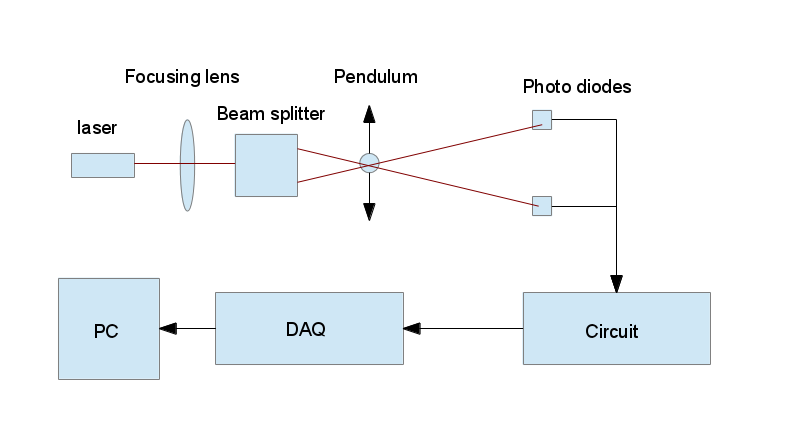
\includegraphics[width=0.8\textwidth]{img/expsetup}
	\caption{Schematic diagram of the experimental set-up. The laser is focused onto the pendulum by the focusing lens. Between focusing lens and the pendulum there is a beam splitter that splits the beam in to two beams that at the pendulum position are very narrowly separated. The photo diodes converts the beam into an electrical signal that goes in to the PC through an ADC.}
	\label{fig:expsetup}
\end{figure}
\begin{figure}[htbp]
	\centering
	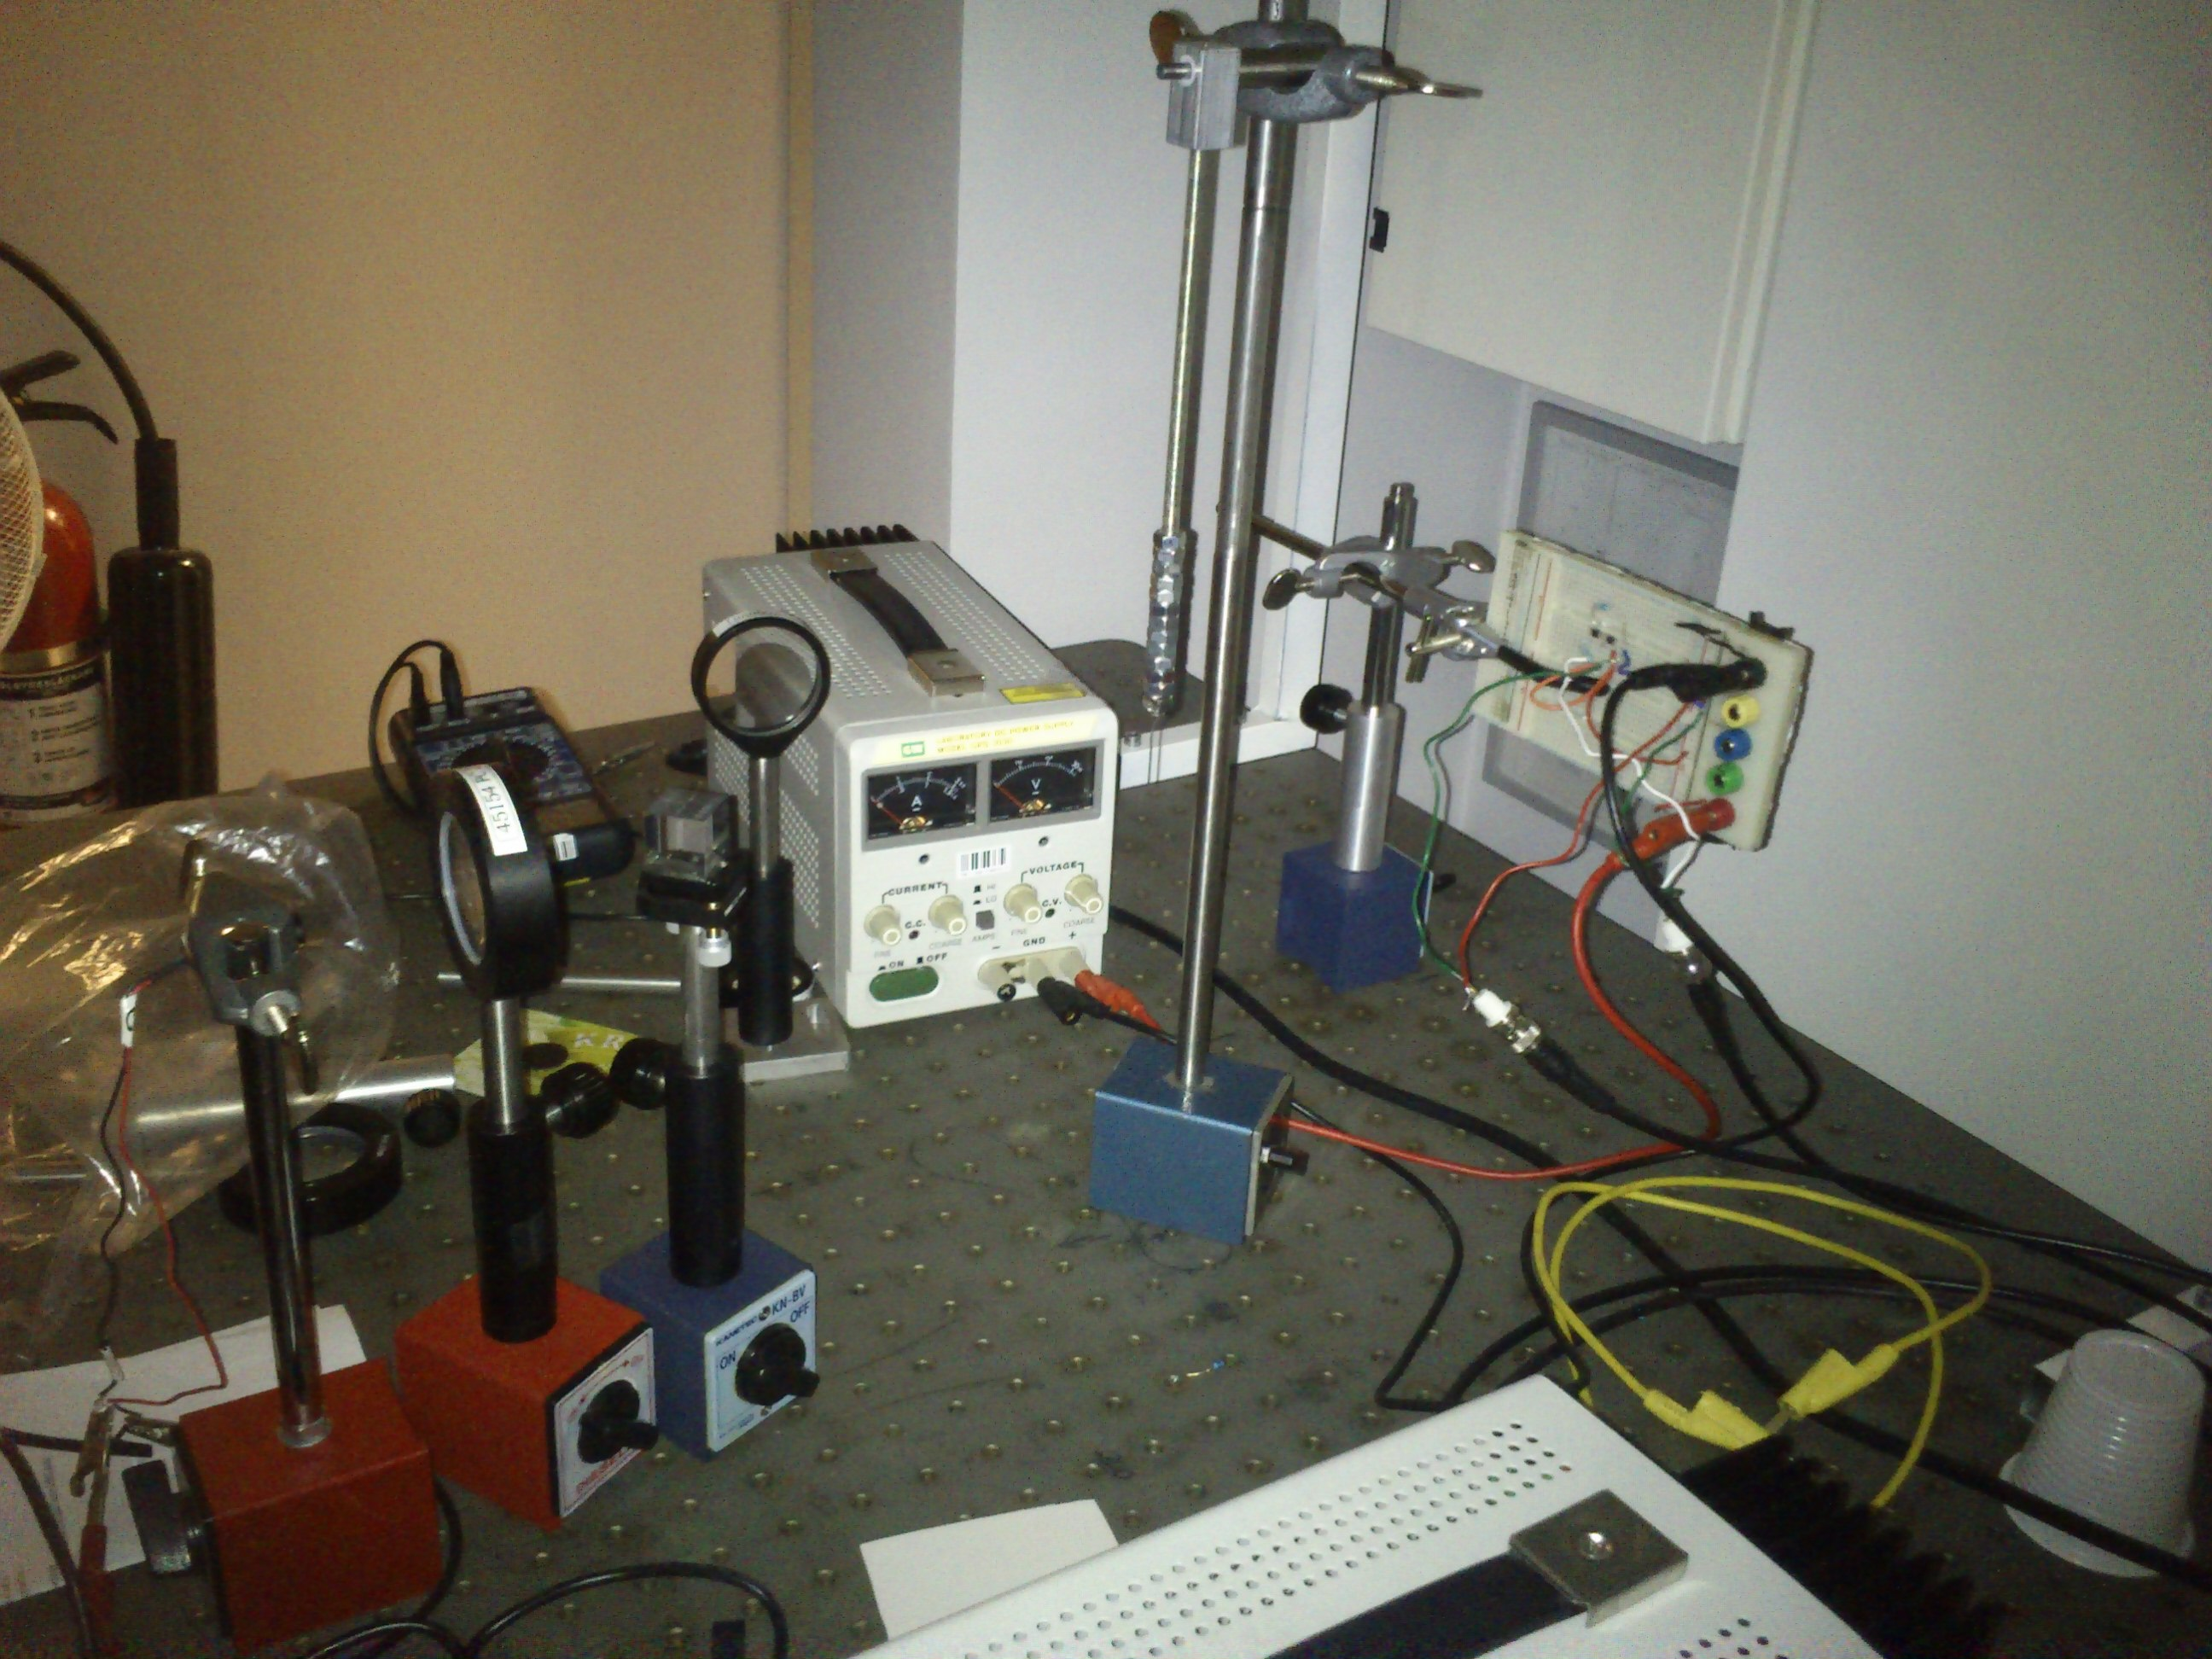
\includegraphics[width=0.8\textwidth]{img/expsetupLive}
	\caption{Real experimental setup. 1. Laser, 2. focusing lens, 3. beam splitter, 4. pendulum,
	5. photo diodes with circuit.} %TODO Add more info, number the components.
	\label{fig:expsetupLive}
\end{figure}
The two laser beams near the pendulum are covered by the pendulum at the different times meaning that there will be valleys in the output signal from the photo diodes at different times.
The velocity of the pendulum will be inversely proportional to the time difference of these two valleys measured by the photo diodes.

The two laser beams are directed at the point where the pendulum has its lowest potential energy or highest kinetic energy; and to get a good value for this velocity the two beams are at this point only separated by a distance of order of a millimetre in length.
Every time the pendulum swings by this point its total energy---which is the same as its kinetic energy---can be calculated and it will decay over time because of energy loss due to air drag and friction.

Since the separation of the two beams is very small we need a high sampling frequency to measure the velocity accurately; we used a sampling frequency of $100\;\rm{kHz}$ which means we can measure velocities in the order of 
%TODO fix this is to much
\mbox{$\approx 1\;\rm{mm} \cdot 100\;\rm{kHz} = 100 \rm{m/s}$}.
But since there is always some noise in the system the velocities which you can distinguish between is lower than this.

To see how the decay in energy of the pendulum depends on the friction, more mass can be added to the pendulum nearly without affecting the air drag, compare fig. \ref{fig:pendulumNormal} and fig. \ref{fig:pendulumHeavy}.
Similarly to examine the energy loss from air drag we changed the geometry of the pendulum, compare
fig. \ref{fig:pendulumNormal} and fig. \ref{fig:pendulumDraggy}.
%\begin{figure}[htbp]
%\begin{subfigure}
%	\centering
%	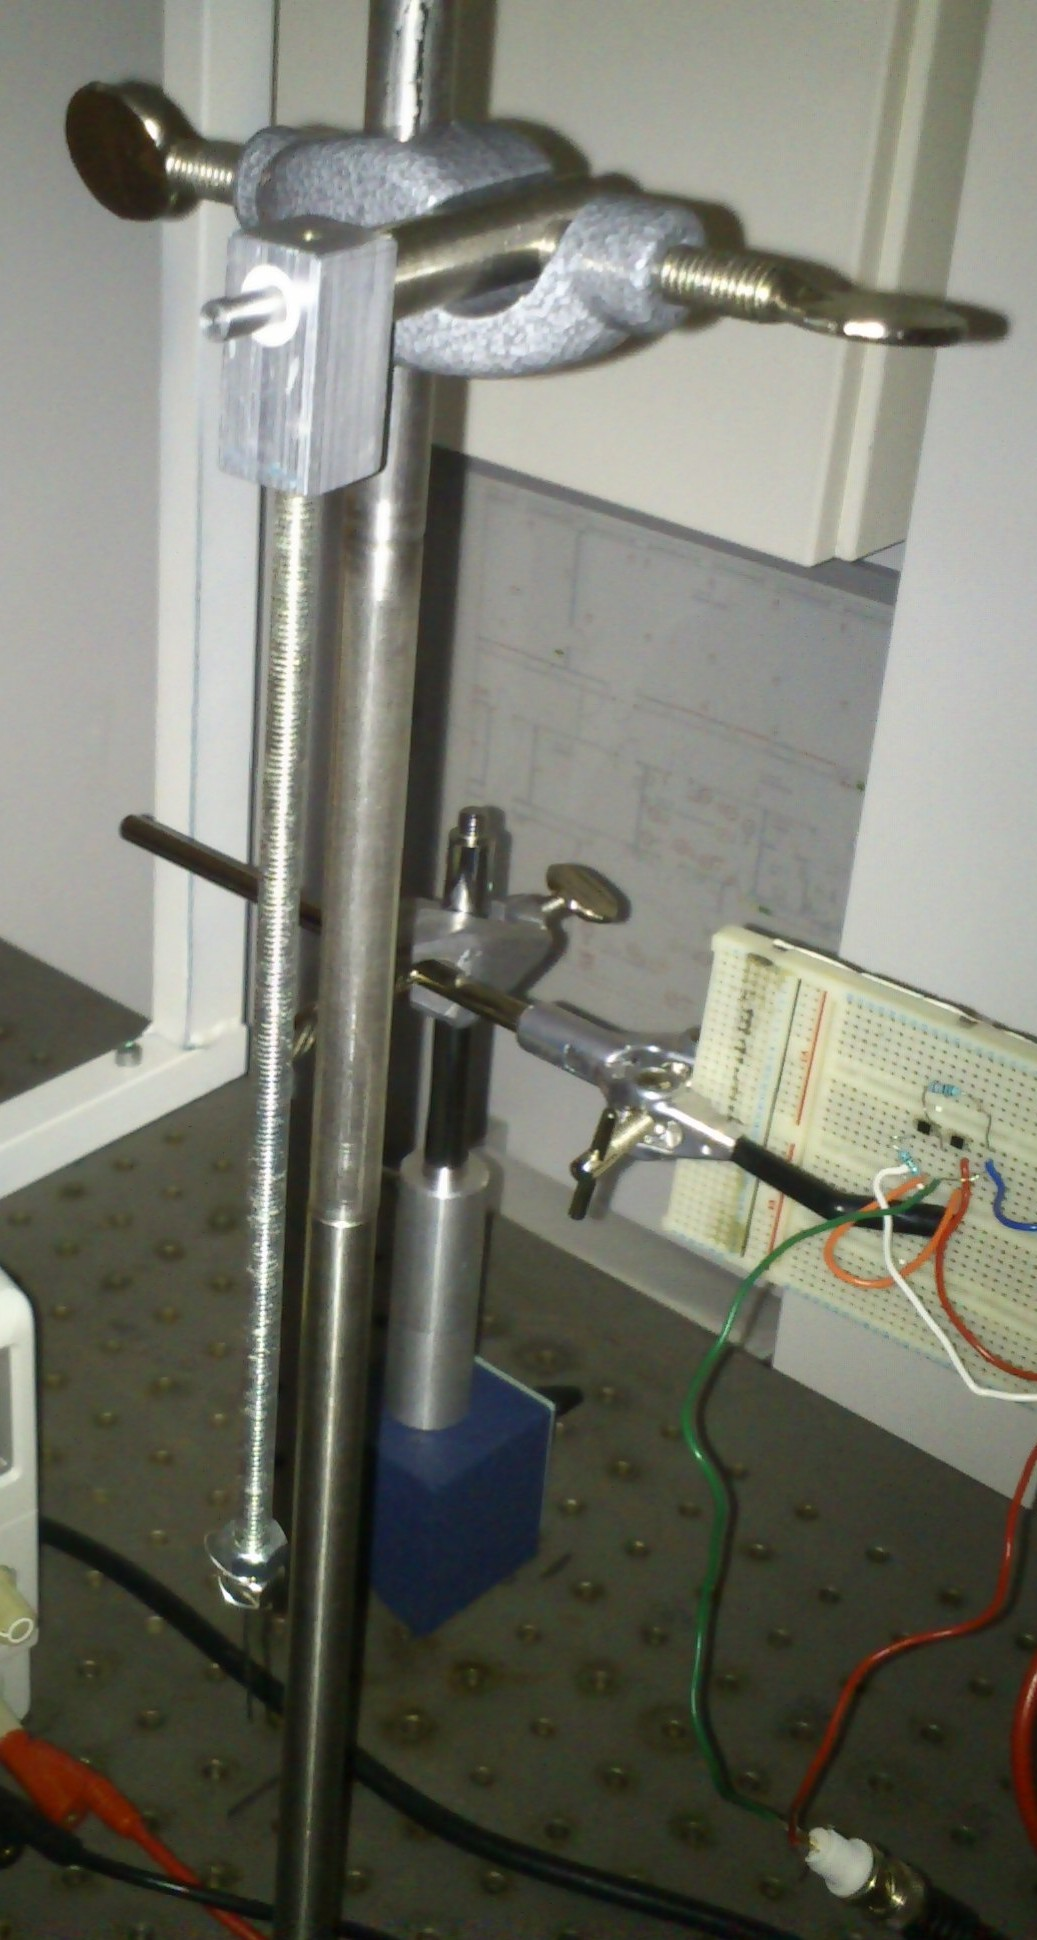
\includegraphics[width=0.50\textwidth]{img/pendulumNormal}
%	\caption{Normal weight and geometry of the  pendulum.}
%	\label{fig:pendulumNormal}
%\end{subfigure}
%\begin{subfigure}
%	\centering
%	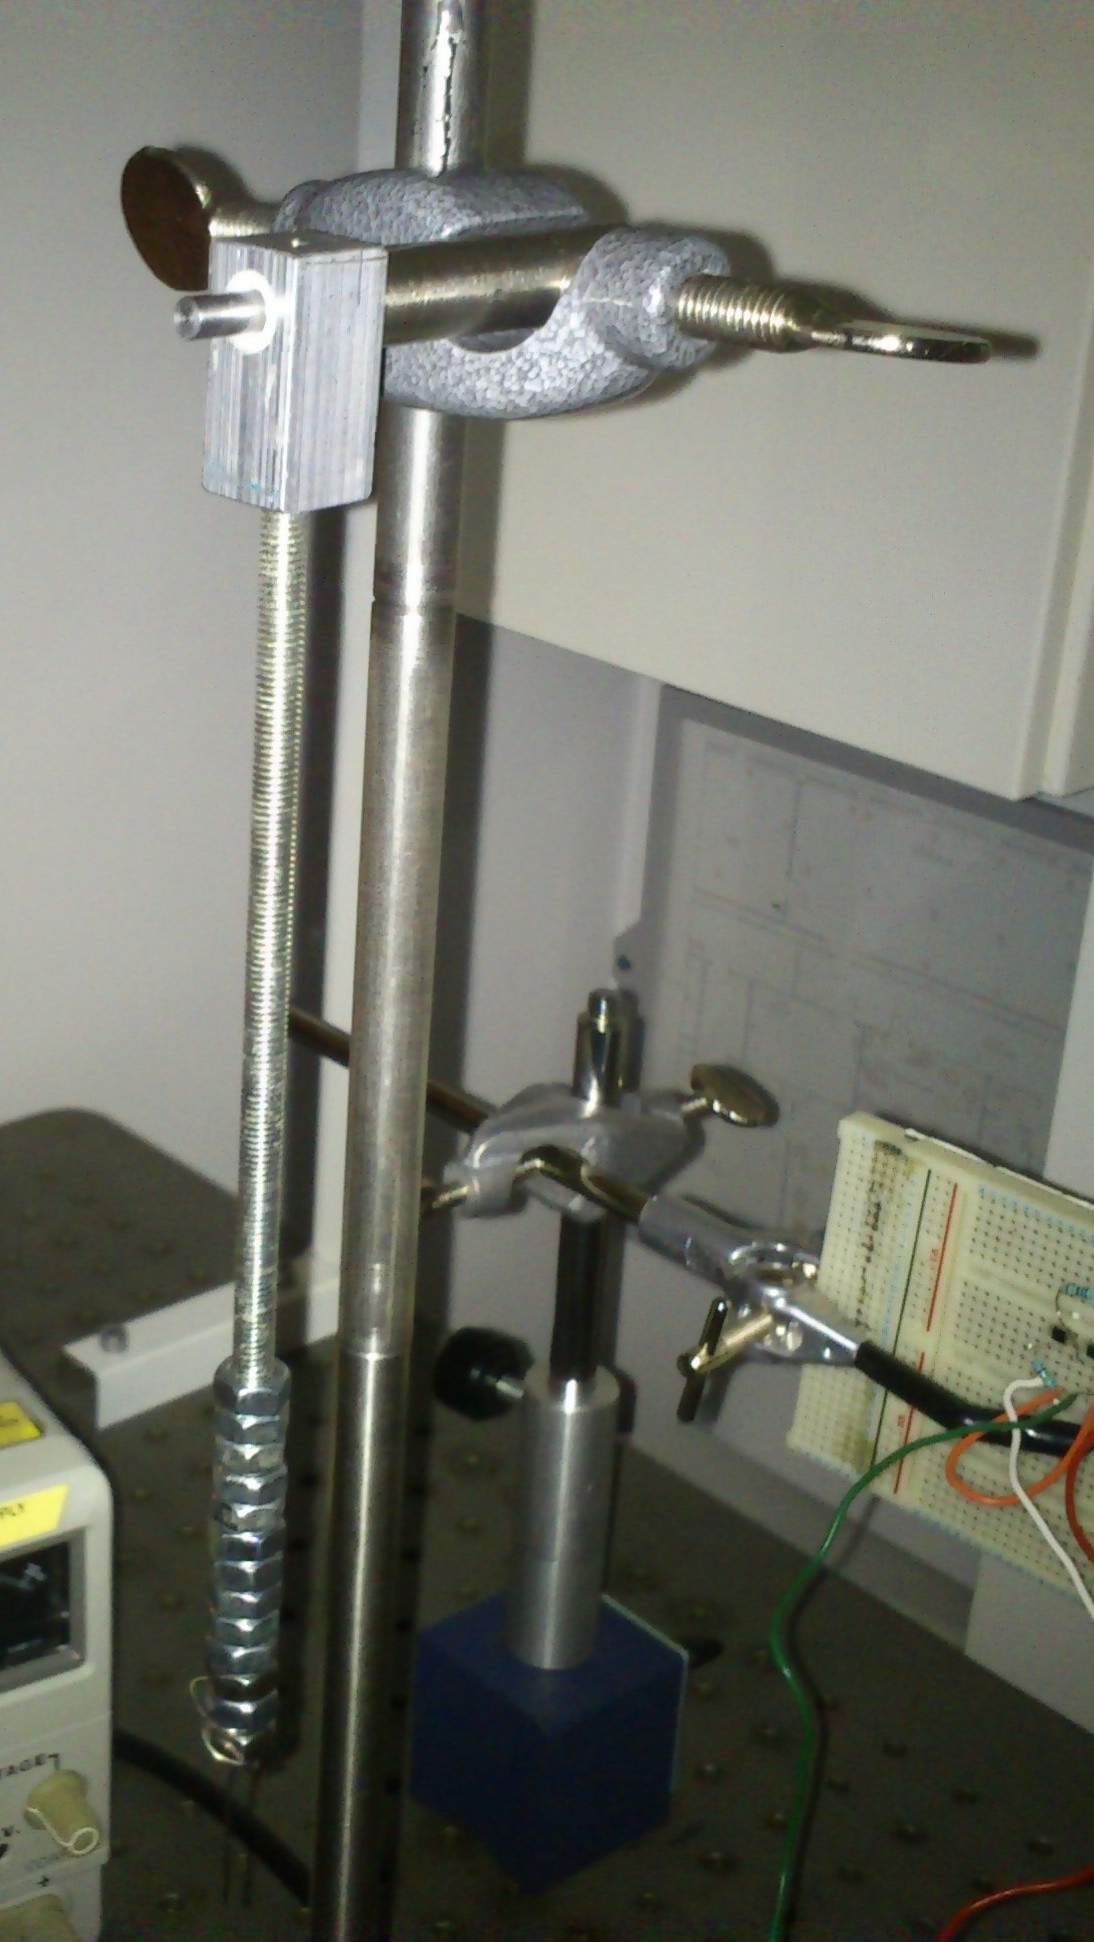
\includegraphics[width=0.50\textwidth]{img/pendulumHeavy}
%	\caption{Pendulum with added mass in the form of screw nuts.}
%	\label{fig:pendulumHeavy}
%\end{subfigure}
%\begin{subfigure}
%	\centering
%	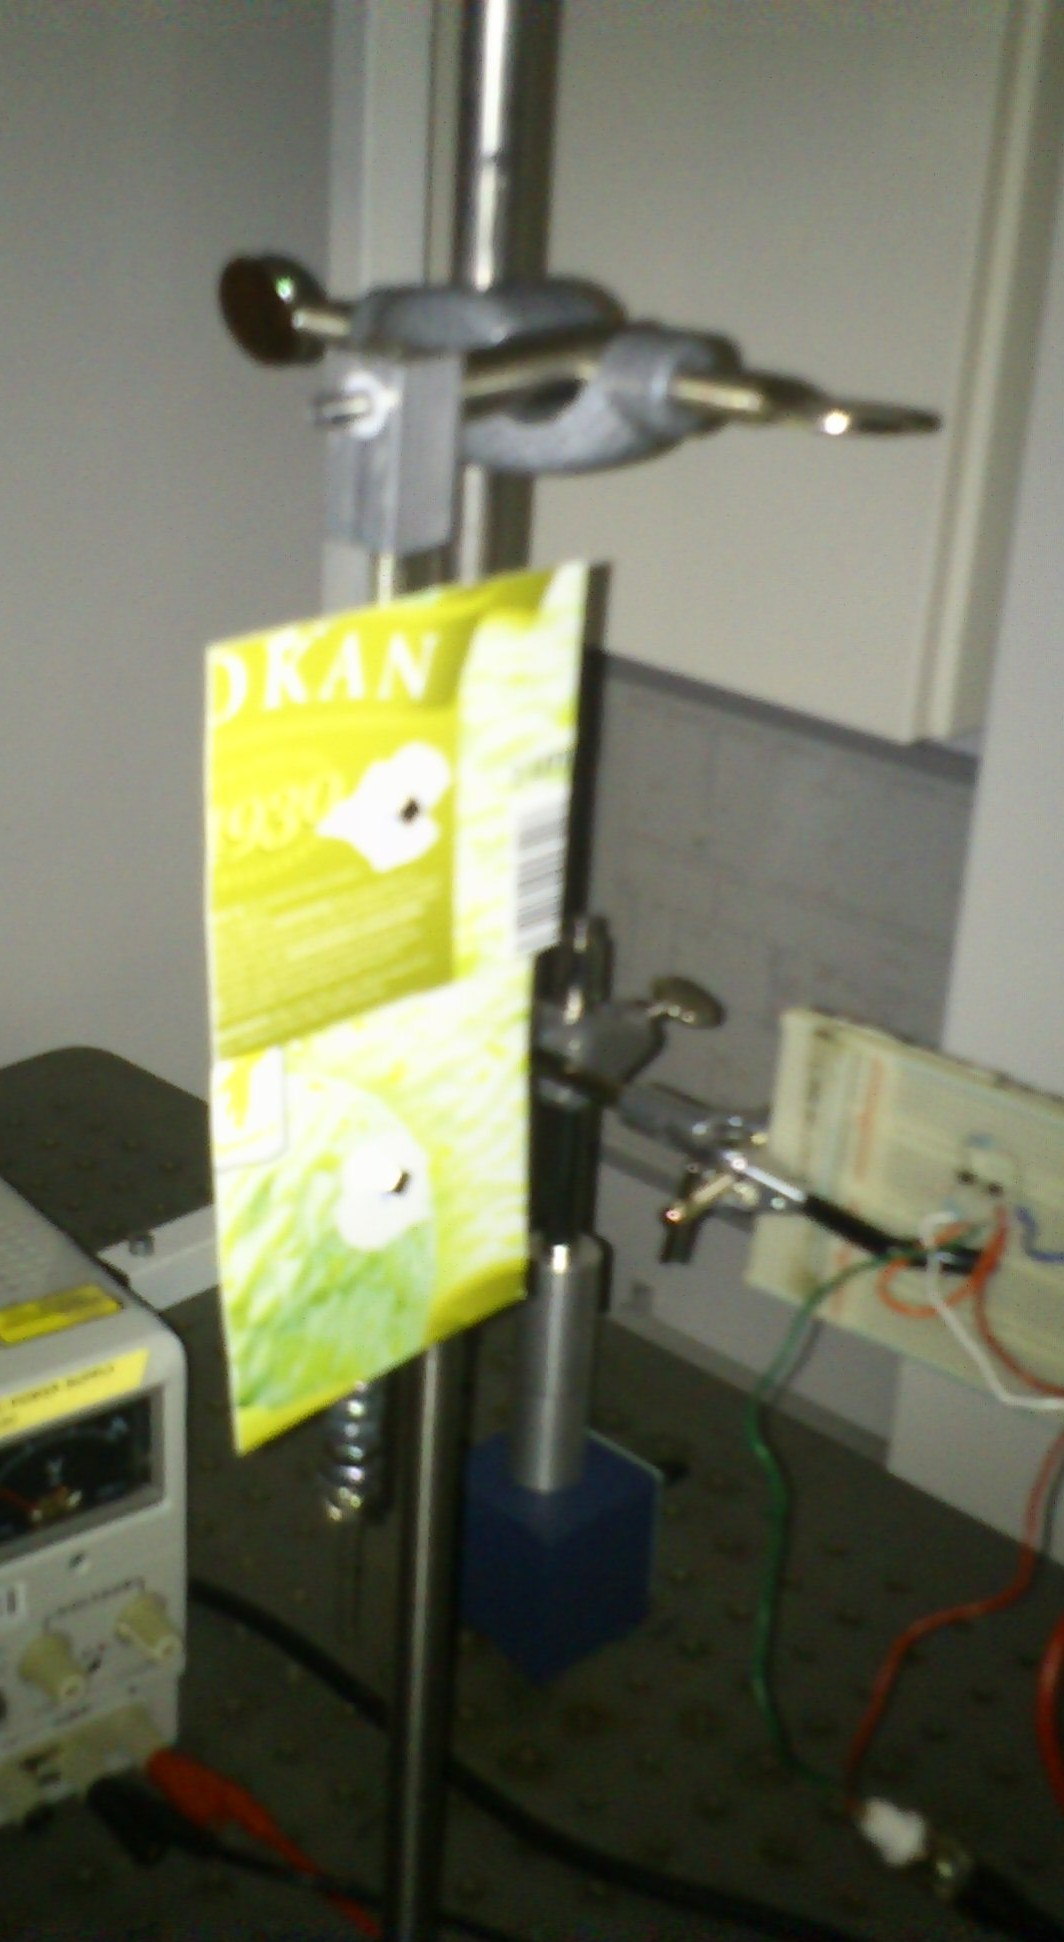
\includegraphics[width=0.50\textwidth]{img/pendulumDraggy}
%	\caption{Pendulum with increased air drag due to changed geometry.}
%	\label{fig:pendulumDraggy}
%\end{subfigure}
%\end{figure}



\begin{figure}[htbp]
\centering
\begin{subfigure}{.3\textwidth}
	\centering
	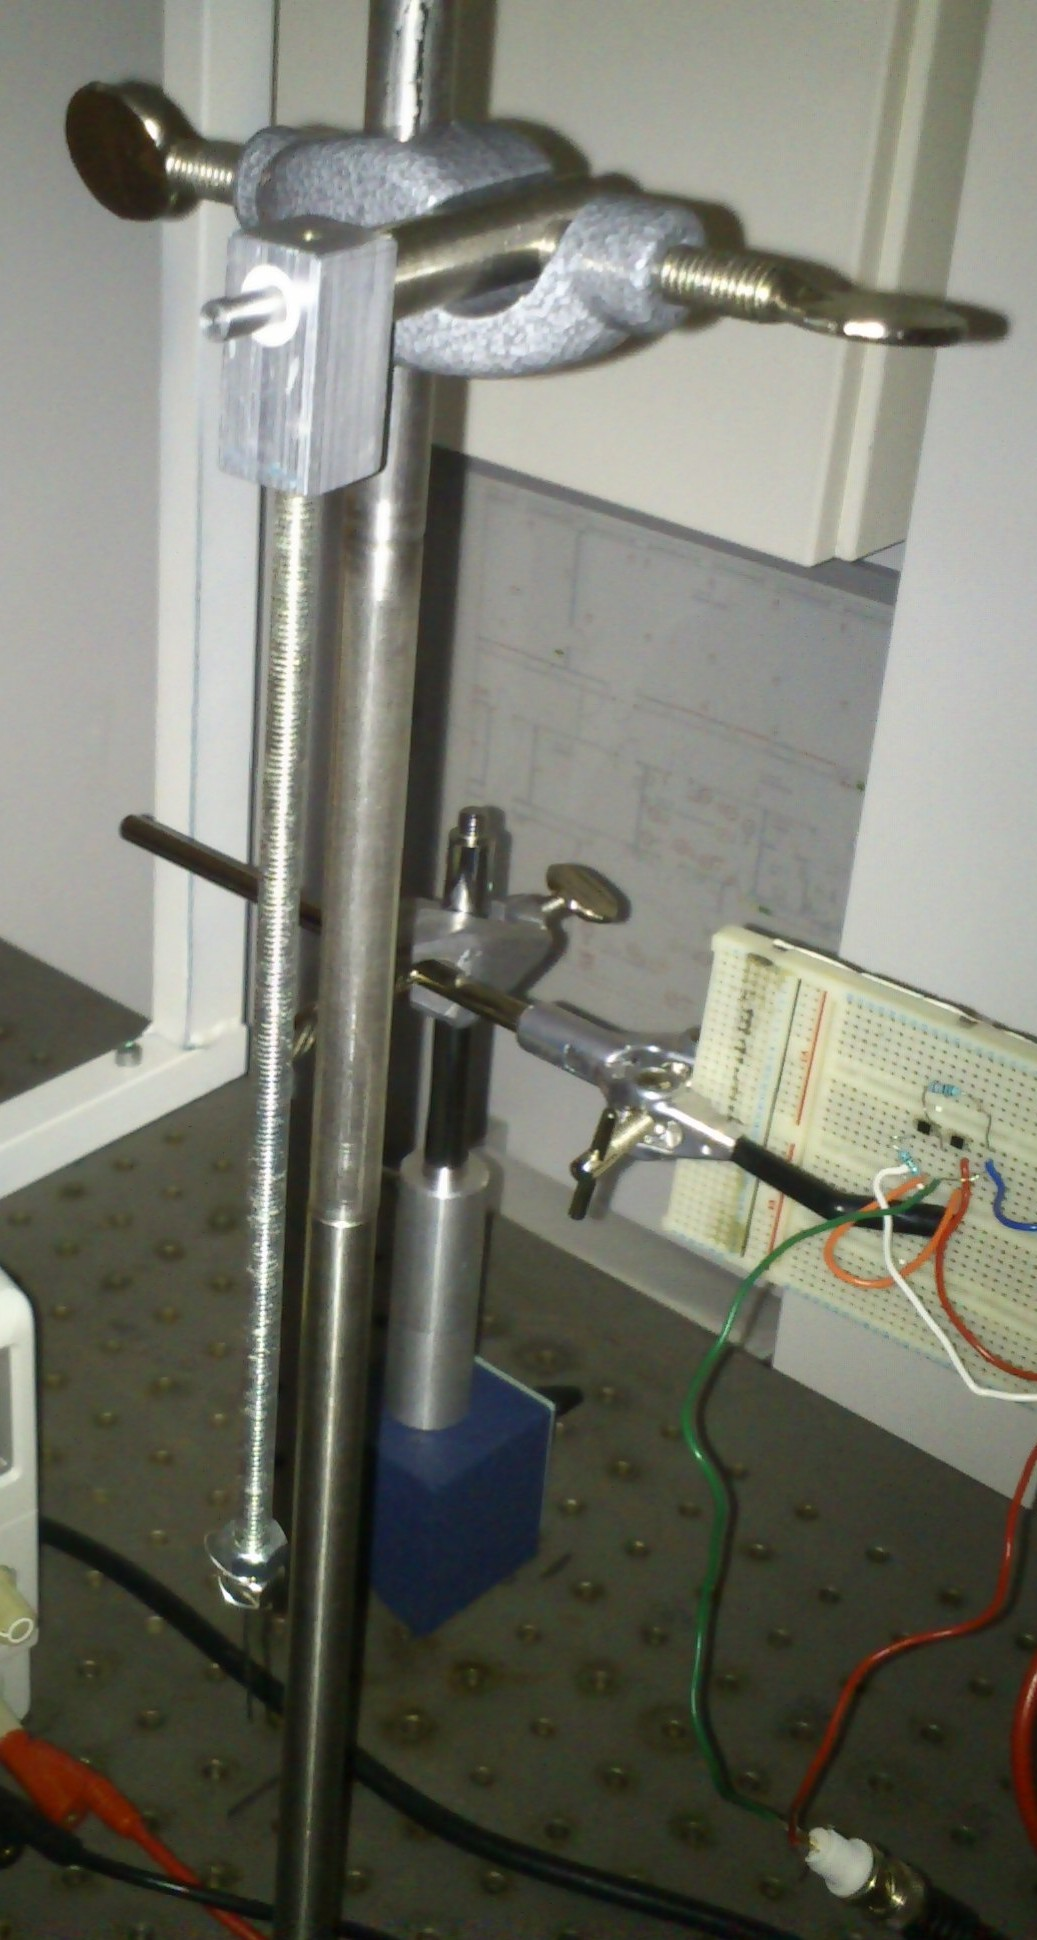
\includegraphics[width=\textwidth]{img/pendulumNormal}
	\caption{}
	\label{fig:pendulumNormal}
\end{subfigure}
\begin{subfigure}{.3\textwidth}
	\centering
	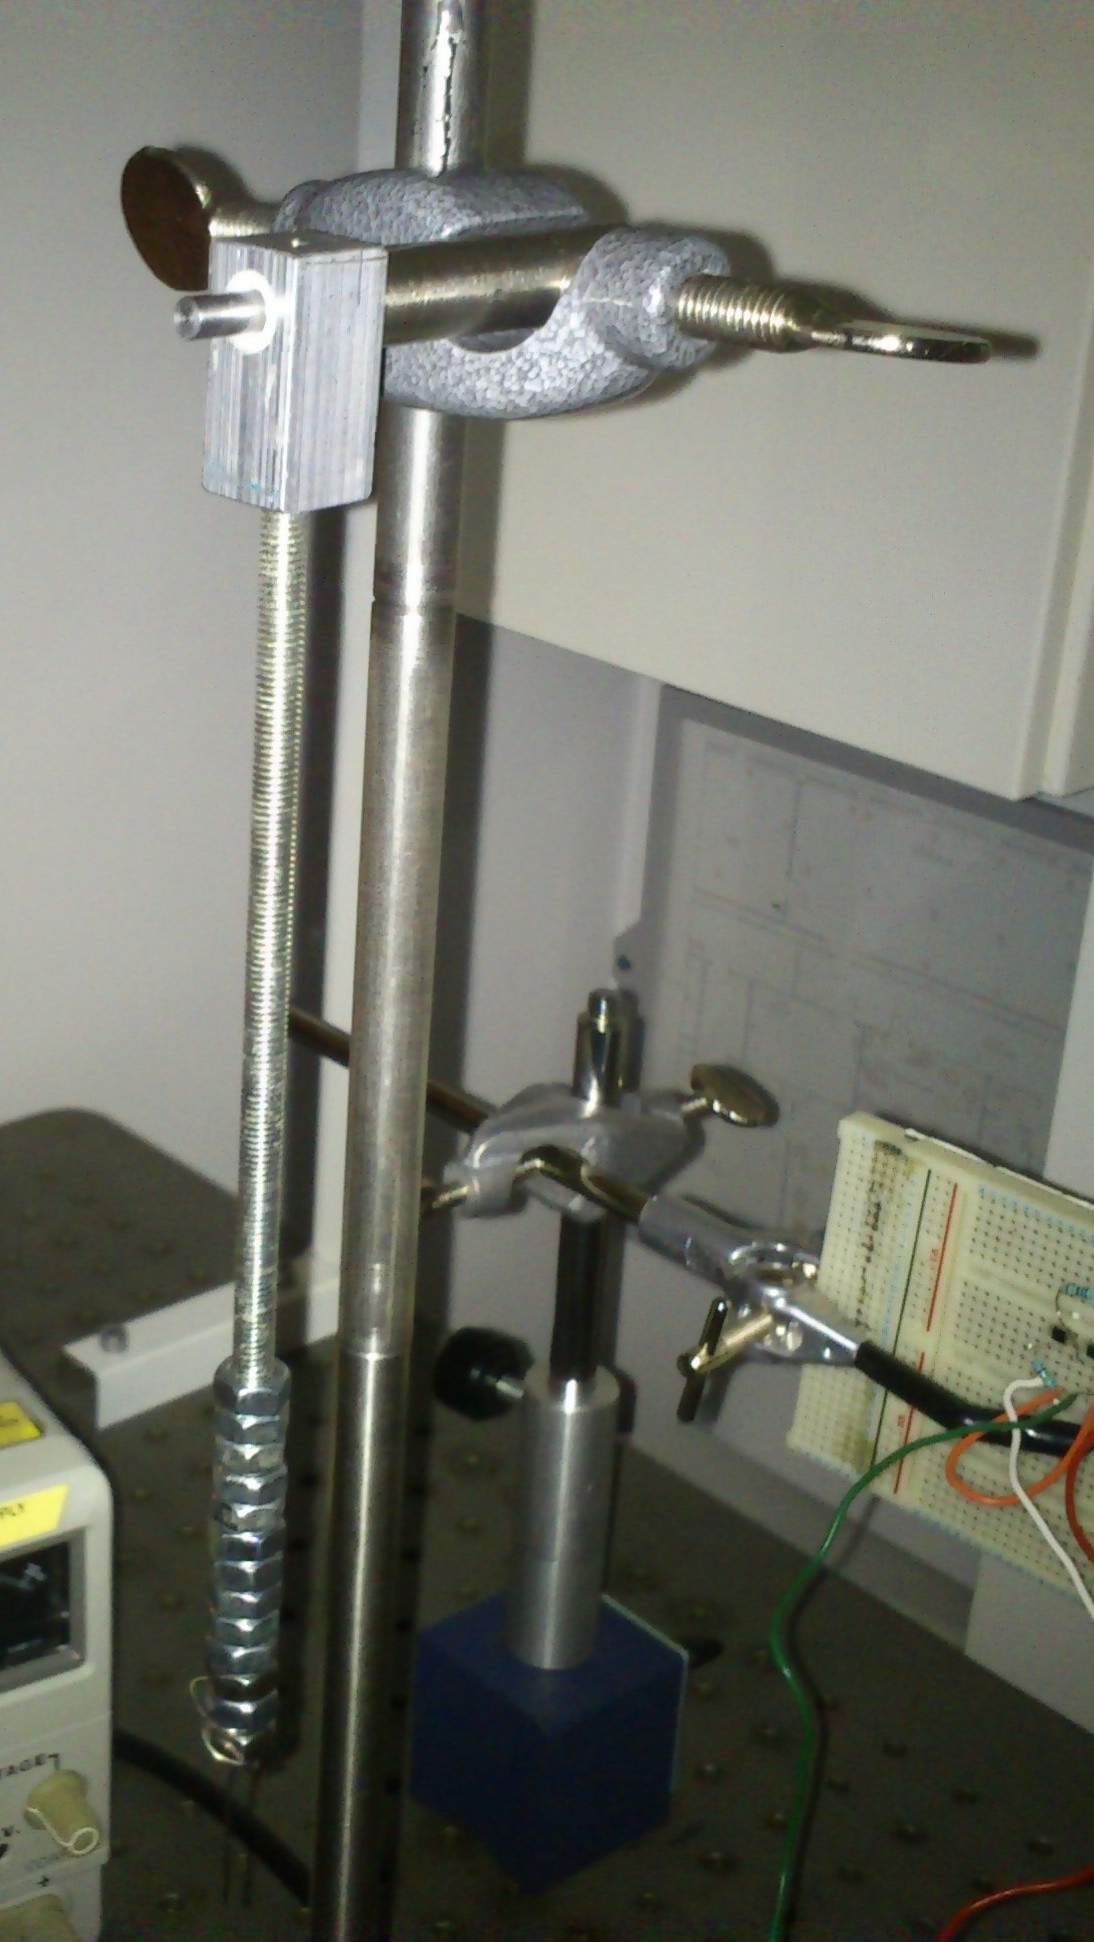
\includegraphics[width=\textwidth]{img/pendulumHeavy}
	\caption{}
	\label{fig:pendulumHeavy}
\end{subfigure}
\begin{subfigure}{.3\textwidth}
	\centering
	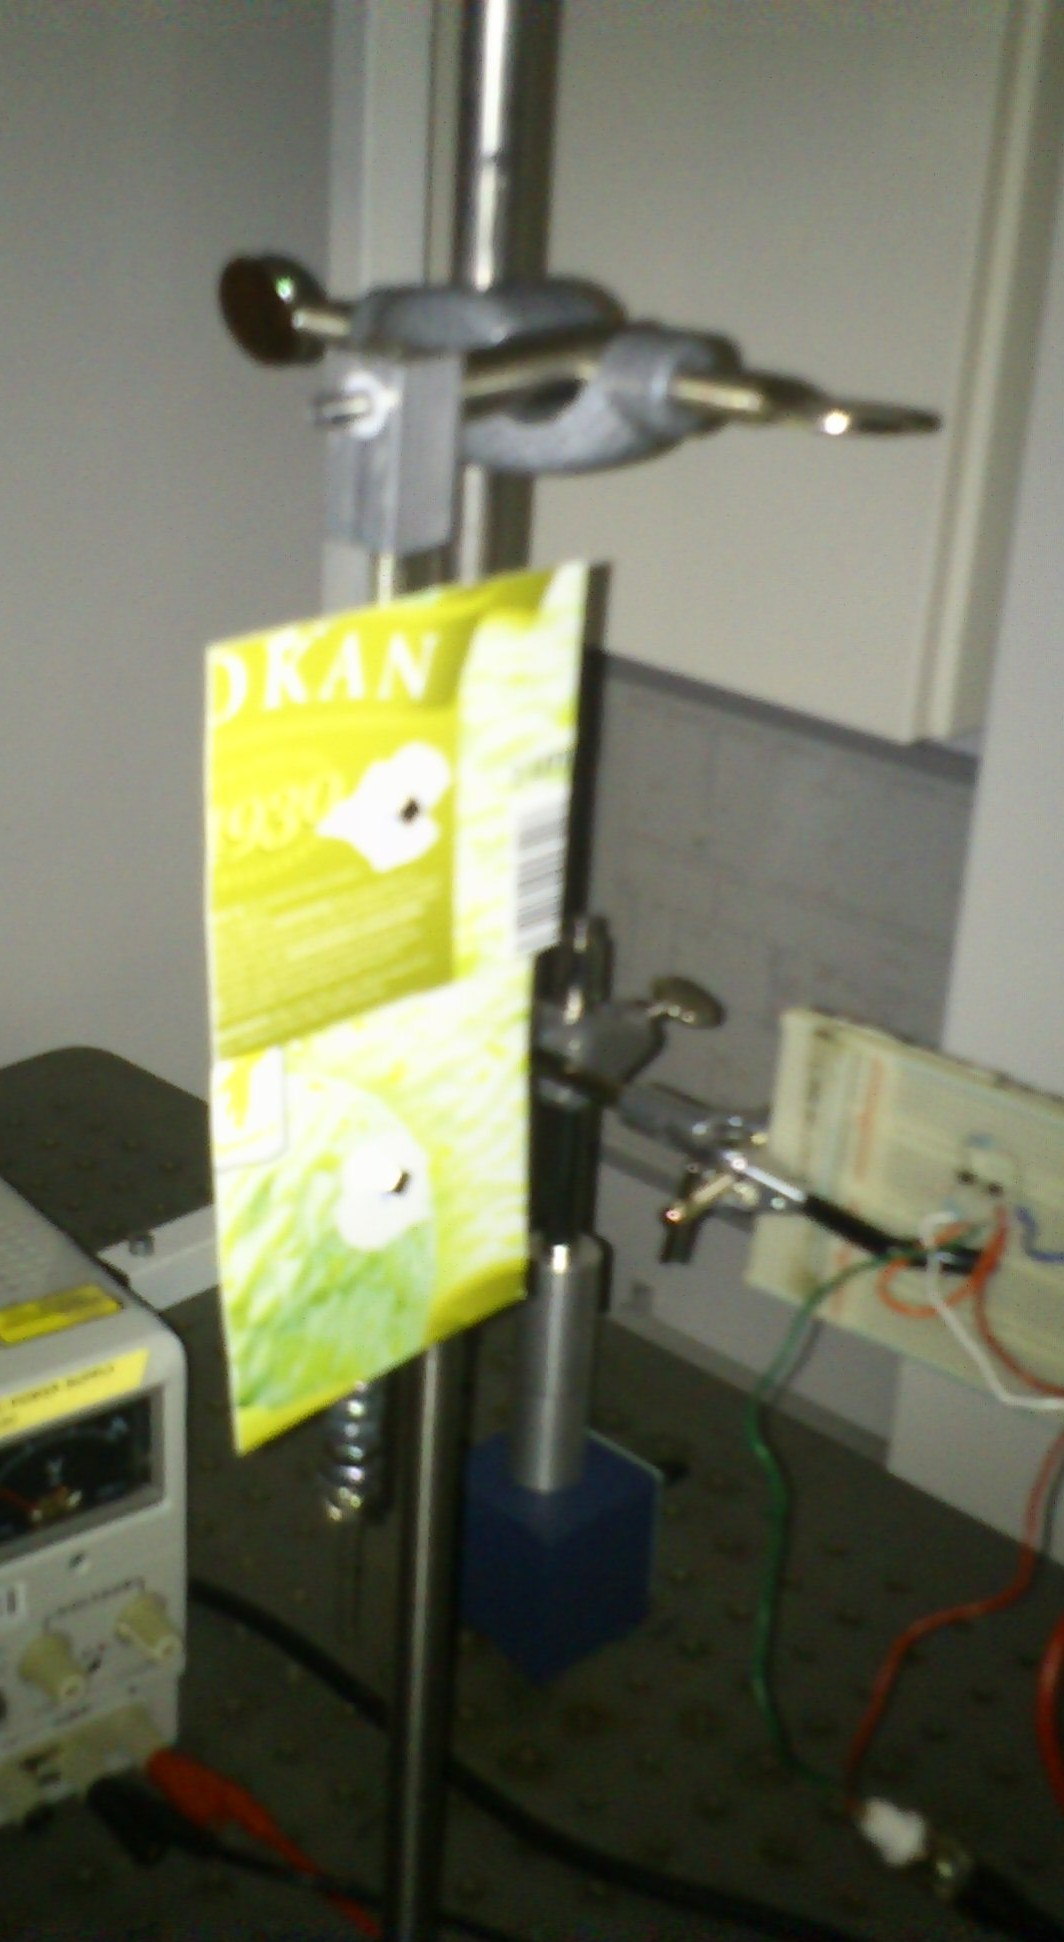
\includegraphics[width=\textwidth]{img/pendulumDraggy}
	\caption{}
	\label{fig:pendulumDraggy}
\end{subfigure}
\caption{(a) Normal weight and geometry of the  pendulum. (b) Pendulum with added mass in the form of screw nuts. (c) Pendulum with increased air drag due to changed geometry.}
\end{figure}

\FloatBarrier
\section{Results}
\subsection{\label{}Oscillation of the tuning fork}

A tuning fork is an acoustic resonator in the shape of a fork with two prongs, forming a U. it is usually made of elastic metal, as f.i. Steel. Apart from the fundamental mode, as illustrated in \ref{fig:tuning}, the tuning fork can also oscillate in higher overtones. Due to the fact, that these higher modes are damped more strongly by the base, they die out faster and leave a a typical pure musical tone. This also causes the short “clang”, that appears when tipping the fork. The pitch of a particular tuning fork depends on the length as well as on the mass of the prongs.

\begin{figure}[H]
	\centering
	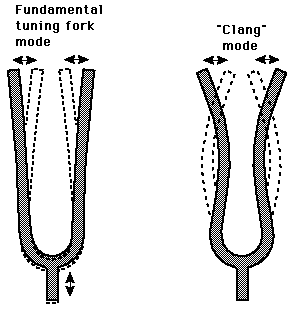
\includegraphics[angle=0,width=0.6\textwidth]{img/tuning}
	\caption{First two balanced modes of a tuning fork.}
	\label{fig:tuning}
\end{figure}

Apart from the modes in which the two prongs oscillate in antiphase, of which the two first are shown in \ref{fig:tuning}, more unbalanced modes exist that transfer onto the base. As the base is in general fixed by holding the tuning fork in the hand or having it fixed by other means, these modes generally don't appear significantly.
The main interest was to measure amplitude and frequency of the vibrations of the tuning fork. To do so, the difference and the sum of the two currents as given out by the electric circuit explained in \ref{} were processed with labview. To calibrate the PSD, the micrometer screw attached to the slide of the tuning fork was used.

In \ref{fig:frequency} the vibration of the tuning fork after 3 seconds of damping is illustrated. The difference of the two currents, that the PSD feeds the electric circuit with, is depicted as a function of the time. As can be seen the tuning fork is harmonically oscillating at a steady frequency.

\begin{figure}[H]
	\centering
	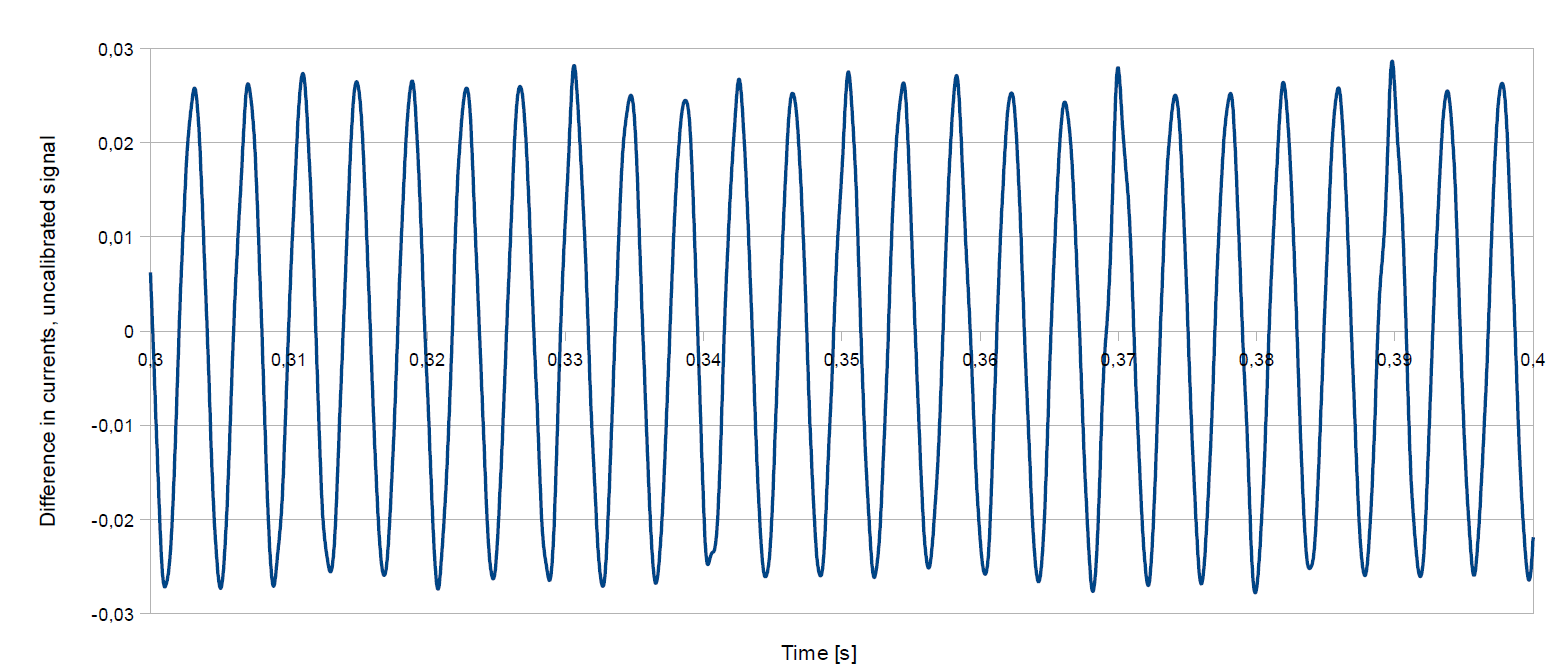
\includegraphics[angle=0,width=0.6\textwidth]{img/frequency}
	\caption{Uncalibrated difference in currents given out by the PSD.}
	\label{fig:frequency}
\end{figure}

This frequency was determined by averaging the periodic time $T$ over 229 periods. Doing this, a frequency of 

\begin{eqnarray}
f = 253,68 Hz
\end{eqnarray}

was found. This gives a relative deviation of $0,9\%$ from the 256 Hz specified by the manufacturer of the tuning fork. Due to the high number of samples a statistic deviation of this magnitude is unlikely.

In \ref{fig:amplitude} the amplitude of the vibration is shown over time. The amplitude was directly calculated from the signal from labview. It can be well seen how after a short phase of transient oscillation withing the first 5 seconds the amplitude decreases very steadily.

\begin{figure}[H]
	\centering
	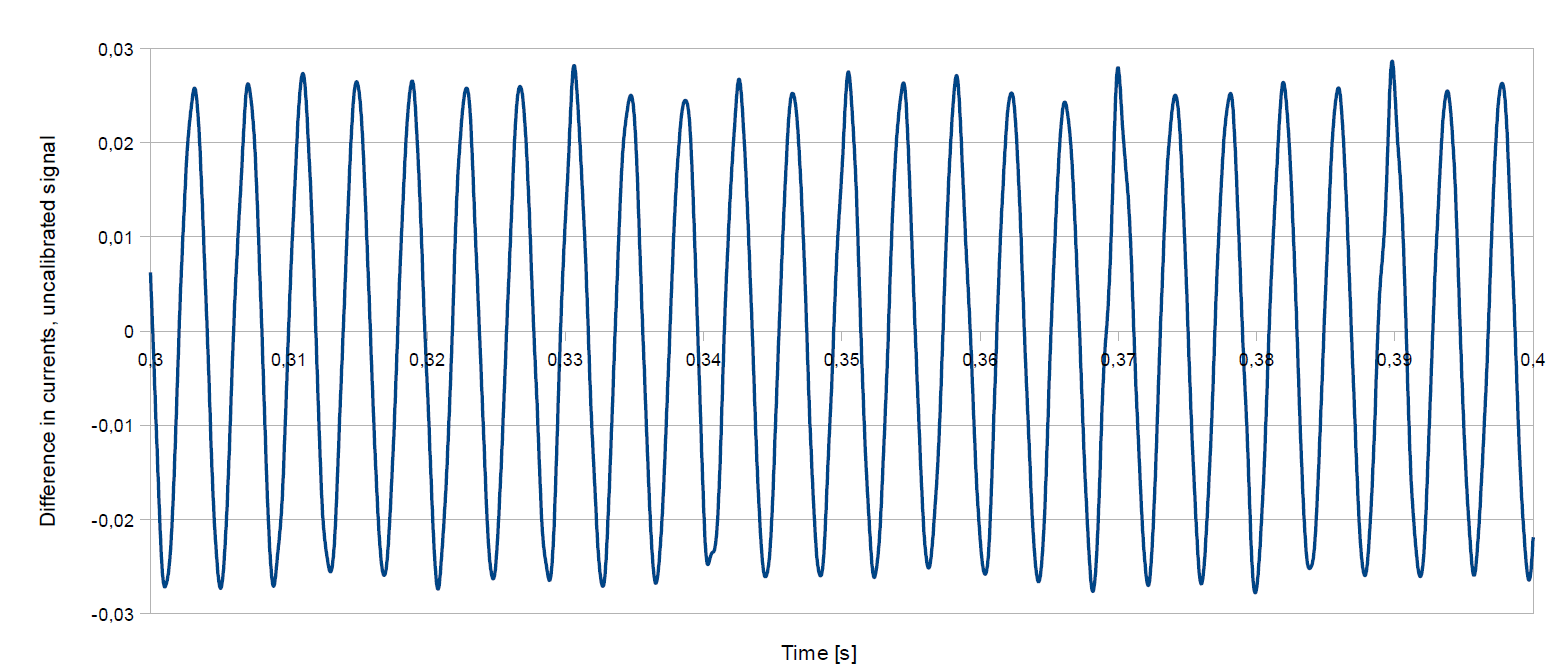
\includegraphics[angle=0,width=0.6\textwidth]{img/frequency}
	\caption{Calibrated amplitude of the oscillations.}
	\label{fig:amplitude}
\end{figure}

Measuring this repeatedly shows that the maximal amplitude highly depends on how hard the tuning fork is stroke, while never exceeding about 0.3 mm and always decreasing in the same way that can me seen in \ref{fig:amplitude}.

\FloatBarrier
\section{Discussion}\label{discussion}
%Function: The function of the Discussion is to interpret your results in light of what was already known about the subject of the investigation, and to explain our new understanding of the problem after taking your results into consideration. The Discussion will always connect to the Introduction by way of the question(s) or hypotheses you posed and the literature you cited, but it does not simply repeat or rearrange the Introduction. Instead, it tells how your study has moved us forward from the place you left us at the end of the Introduction.

%1. Do your results provide answers to your testable hypotheses? If so, how do you interpret your findings?

%2. Do your findings agree with what others have shown? If not, do they suggest an alternative explanation or perhaps a unforseen design flaw in your experiment (or theirs?)

%3.Given your conclusions, what is our new understanding of the problem you investigated and outlined in the Introduction?


%4. If warranted, what would be the next step in your study, e.g., what experiments would you do next?
To get a better picture of the expected results of this experiment we identified the metals the rods were constituted of. This was done by measuring the densities of both rods and comparing it to tabulated values. From this we found rod 1 to be made out of aluminium and rod 2 to be made out of titanium.\\

After the rods where identified we could also look up their respective linear thermal expansion coefficients.
For the aluminium rod the tabulated value were $23\cdot10^{-6} \rm{1/K}$ \cite{coff}. This is outside the measured value of $26.605 \cdot 10^{-6} \pm 0.416 \cdot 10^{-6} \; \rm{1/K}$ which indicate some systematic error.
For the titanium rod which has a tabulated coefficient of linear thermal expansion of $8.6\cdot10^{-6} \rm{1/K}$ \cite{coff}; we see that our calculated value of about $19.371 \cdot 10^{-6} \pm 0.110 \cdot 10^{-6} \; \rm{1/K}$ is not reasonable either.\\

One of the main reasons why our measurements suffered significant errors could possibly be due to an uneven temperature gradient in both the radial and axial direction. As a result the temperature measurements we got from the thermistors will not give a good representation of the rods true temperature.


\FloatBarrier
\section{Conclusions}
To get better results we need to determine the temperature distribution much better.
One problem was that the thermistors only measured the temperature at three points on the surface of the metal. Then we assumed that the temperature gradient was linear between the measured points and that the temperature was the same in the core of the rod as on the surface. We don't have any error estimate of how large this error might be and if it might explain why the results did not correspond with tabulated values.

%\begin{appendix}
%
%\section{Appendix section 1}
%%Here you can put additional data of importance Labview or Matlab codes,
%%additional equations and derivations etc.
%%Do not add long tables of raw data. 
%%
%%For programming code like Matlab you need to use a font where 
%%all letters are equally wide. Use the verbatim environment.
%%
%%\begin{verbatim}
%%	Paste code here! 
%%\end{verbatim}
%
%\section{Appendix section 2} 
%	
%\end{appendix}

\bibliographystyle{plain}

\begin{thebibliography}{99}
	%Vink, G. E., Morgan, W. J., and Vogt, P. R., 1985, The Earth's hot spots, Scientific American, v. 252, p. 50- 57.
%	\bibitem{Franca05} Franca, J.G.D.M.; Gazziro, M.A.; Ide, A.N.; Saito, J.H.; 2005, A 3D scanning system based on laser triangulation and variable field of view, \emph{IEEE International Conference On Image Processing}, v.1 p.859-866.
%	
%	\bibitem{Matthies97} Matthies, L., Balch, T. and Wilcox, B, 1997, Fast optical hazard detection for planetary rovers using multiple spot laser triangulation, \emph{IEEE International Conference On Robotics And Automation}, I-425-8.
%
%	\bibitem{Okkerse00} Okkerse W.J.H., Ottengraf S.P.P., Osinga-Kuipers B., 2000, Biofilm thickness variability investigated with a laser triangulation sensor, \emph{Biotechnology and Bioengineering} v.70 p.619-629.	
	%\bibitem{ref2} author1 and author2, Book title, Publisher, Country, (year) . 
		
%	\bibitem{coilImpedance} An introduction to Eddy Current Testing, Jospeh M. Buckley, \url{http://joe.buckley.net/papers/eddyc.pdf}(2013/Dec/06) 
%
%	\bibitem{eddyCurrent} Non-Destructive Techniques Based on Eddy Current Testing, Javier García-Martín et al., \url{http://www.ncbi.nlm.nih.gov/pmc/articles/PMC3231639/}(2013/Dec/06) 
%
%	\bibitem{feromagnetism} Magnetische Permeabilität der ferromagnetischen Metalle bei sehr hoher Frequenz, G. Potapengo., \url{http://download.springer.com/static/pdf/156/art\%253A10.1007\%252FBF01504219.pdf?auth66=1386496540_e2473c0e5366f59d74fc10eeb80accef&ext=.pdf}(2013/Dec/06)
%	
%		\bibitem{deedsdodd} C. V. Dodd, W. E. Deeds, 1968, Analytical Solutions to Eddy-Current Probe-Coil Problems, \emph{Journal of applied physics} v.39 p.2829-2838.
\bibitem{torque} Torque, \url{http://en.wikipedia.org/wiki/Torque}, (\today).
\bibitem{friction} Dry friction, \url{http://en.wikipedia.org/wiki/Friction#Dry_friction}, (\today).
\bibitem{centripetalforce} Centripetal force, \url{http://en.wikipedia.org/wiki/Centripetal_force}, (\today).
\bibitem{airdrag} Air drag, \url{http://en.wikipedia.org/wiki/Air_drag}, (\today).
\end{thebibliography}



\end{document}